\documentclass[11pt, a4paper, twoside]{article}   	% use "amsart" instead of "article" for AMSLaTeX format

\usepackage{geometry}                		% See geometry.pdf to learn the layout options. There are lots.
\usepackage{pdfpages}
\usepackage{caption}
\usepackage{minted}
\usepackage[german]{babel}			% this end the next are needed for german umlaute
\usepackage[utf8]{inputenc}
\usepackage{color}
\usepackage{graphicx}
\usepackage{titlesec}
\usepackage{fancyhdr}
\usepackage{lastpage}
\usepackage{hyperref}
\usepackage[autostyle=false, style=english]{csquotes}
\usepackage{mathtools}
\usepackage{tabularx}
% http://www.artofproblemsolving.com/wiki/index.php/LaTeX:Symbols#Operators
% =============================================
% Layout & Colors
% =============================================
\geometry{
   a4paper,
   total={210mm,297mm},
   left=20mm,
   right=20mm,
   top=20mm,
   bottom=30mm
 }	

\definecolor{myred}{rgb}{0.8,0,0}
\definecolor{mygreen}{rgb}{0,0.6,0}
\definecolor{mygray}{rgb}{0.5,0.5,0.5}
\definecolor{mymauve}{rgb}{0.58,0,0.82}

\setcounter{secnumdepth}{4}


% the default java directory structure and the main packages
\newcommand{\srcEmit}{../src/Reflection.Emit.Solution/Reflection.Emit}
\newcommand{\srcSymbolic}{../src/Reflection.Emit.Solution/Symbolic.Computation}
\newcommand{\imageDir}{images}
% =============================================
% Code Settings
% =============================================
\newenvironment{code}{\captionsetup{type=listing}}{}
\newmintedfile[cppSourceFile]{cpp}{
	linenos=true, 
	frame=single, 
	breaklines=true, 
	tabsize=2,
	numbersep=5pt,
	xleftmargin=10pt,
	baselinestretch=1,
	fontsize=\footnotesize
}

\newcommand{\xvdash}[1]{%
  \vdash^{\mkern-10mu\scriptscriptstyle\rule[-.9ex]{0pt}{0pt}#1}%
}

% =============================================
% Page Style, Footers & Headers, Title
% =============================================
\title{Übung 3}
\author{Thomas Herzog}

\lhead{Übung 3}
\chead{}
\rhead{
\includegraphics[scale=0.10]{FHO_Logo_Students.jpg}}

\lfoot{S1610454013}
\cfoot{}
\rfoot{ \thepage / \pageref{LastPage} }
\renewcommand{\footrulewidth}{0.4pt}
% =============================================
% D O C U M E N T     C O N T E N T
% =============================================
% =============================================
% 2016.10.13: 1 
% 2016.10.14: 2
% =============================================
\pagestyle{fancy}
\begin{document}
\setlength{\headheight}{15mm}
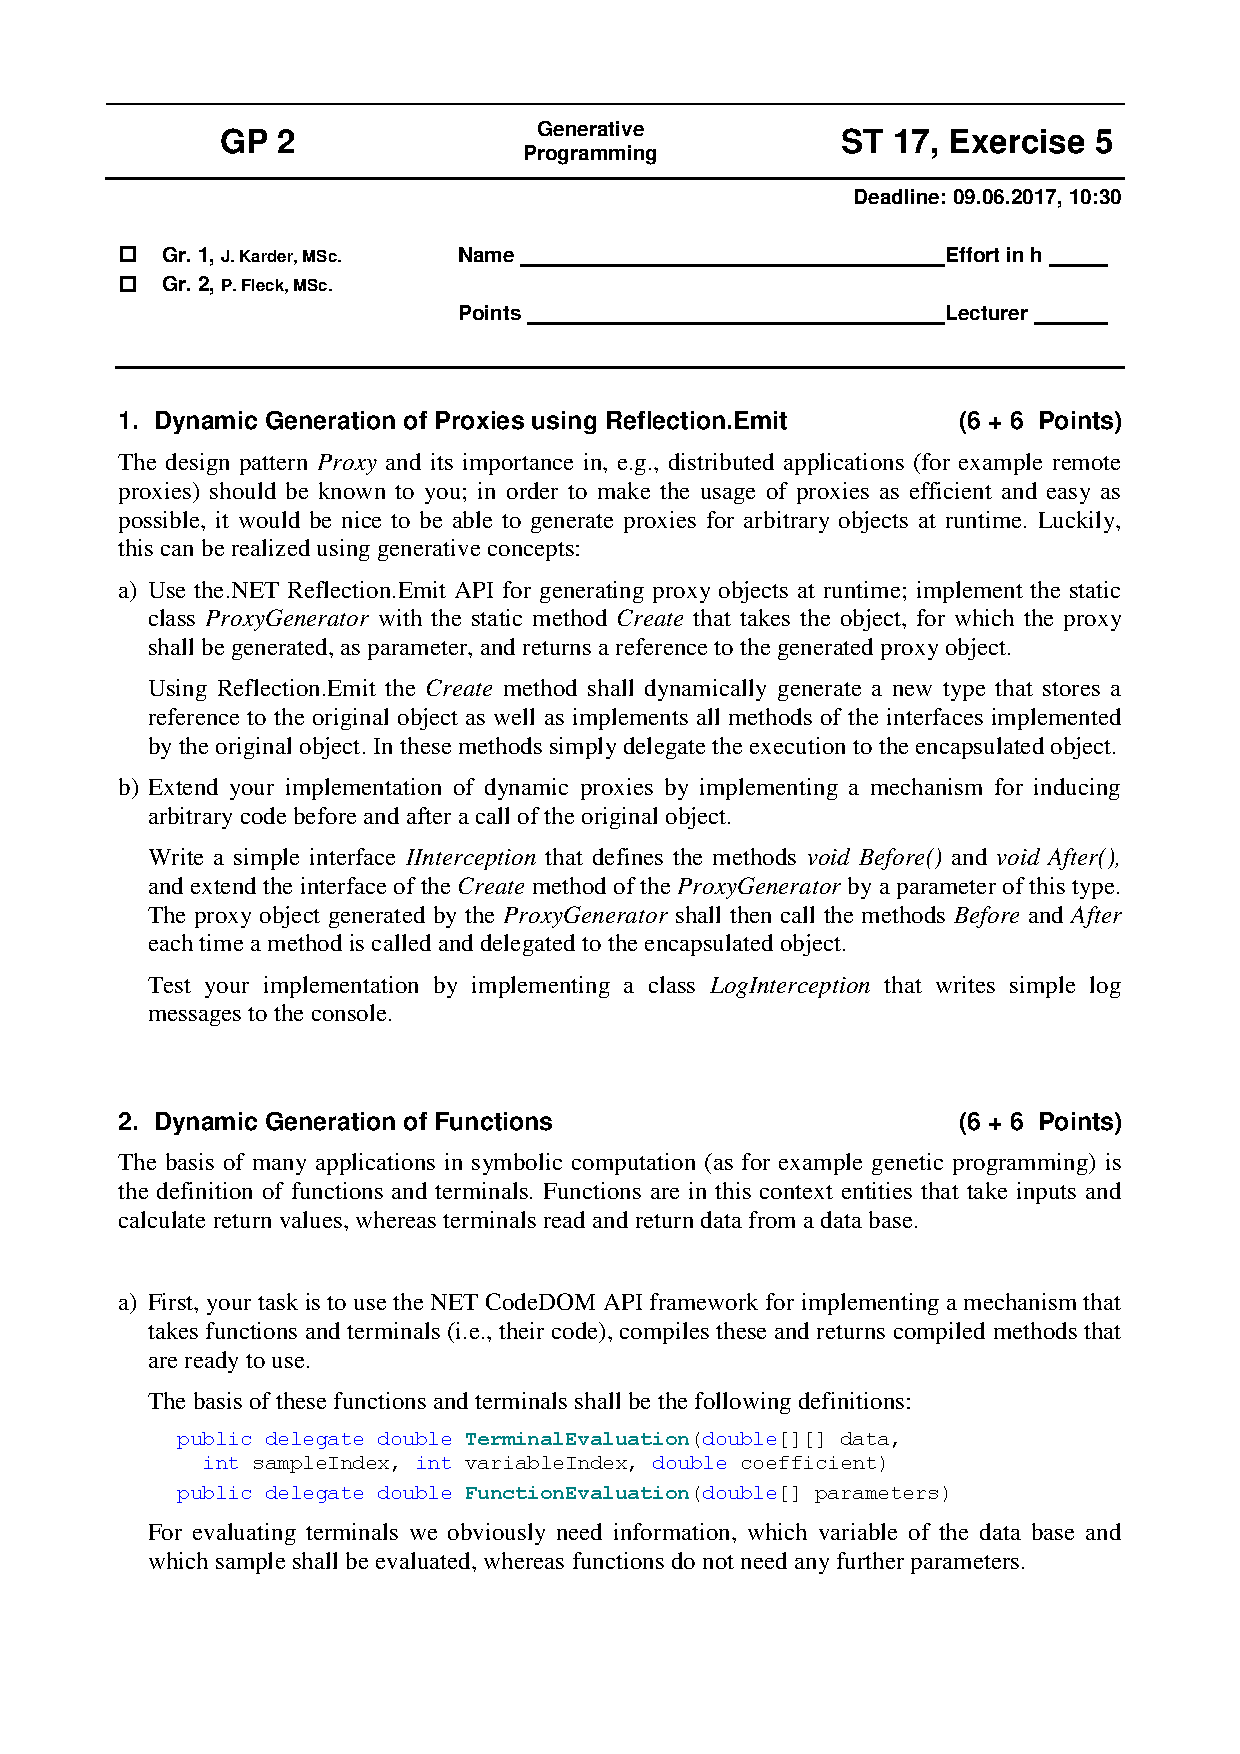
\includepdf[pages={1,2}]{GP_A05.pdf}

\section{Dynamic Generation of Proxies using Reflection.Emit}
Dieser Abschnitt behandelt die Aufgabenstellung \emph{Dynamic Generation of Proxies using Reflection.Emit}.

\subsection{Lösungsidee} 
Es wird die Klasse \emph{ProxyGenerator} implementiert, welche die beiden generischen Methoden \emph{Create$<T>$(T obj)} und \emph{Create$<T>$(T obj, IInterception$<T>$ interceptor)} zur Verfügung stellt, die für das übergebene Objekt eine Proxyklasse und ein Proxyobjekt erstellen und das erstellte Proxyobjekt zurückliefern. Damit der Proxy auch bei einem \emph{Cast} auf den implementierten Typ greift, müssen die implementierten Methoden der Schnitstelle in der implementierenden Klasse als \emph{virtual} markiert werden, ansonsten wird die Implementierung implementierenden Klasse aufgerufen und nicht die überschriebenen Methoden des Proxy, was an der Art und Weise der Handhabung von der dynamischen Bindung in C\# liegt.
\newline
\newline
Es werden alle Methoden im Proxy überschrieben, jedoch wird der \emph{Interceptor} nur bei den Methoden, die im Typ \emph{T} zur Verfügung stehen eingefügt. Ein Interceptor wird durch die Schnittstelle \emph{IIntercepton} spezifiziert, wobei die beiden Methoden \emph{Before} und \emph{After} von einem \emph{Interceptor} implementiert werden müssen. Diese beiden Methoden \emph{Before} und \emph{After} bekommen das Objekt vom Typ \emph{T} und den Methodennamen übergeben, sodass der \emph{Interceptor} mit dem Objekt interagieren kann und auch die Information hat welche Methode abgefangen wird.
\newline
\newline
Es wird die Klasse \emph{LogInterception} implementiert, welche die Schnittstelle \emph{IInterception} implementiert und bei einem Aufruf der Methoden \emph{Before} und \emph{After} \emph{Logs} generiert.

\subsection{Quelltexte}
Dieser Abschnitt beinhaltet die implementierten Quelltexte und das Testprogramm.
\begin{code}
	\caption{IInterception.cs}
	\cppSourceFile{\srcEmit/IInterception.cs}
	\label{src:interface-iinterception}
\end{code}

\begin{code}
	\caption{Interfaces.cs}
	\cppSourceFile{\srcEmit/Interfaces.cs}
	\label{src:interface-itest-isecondtest}
\end{code}

\begin{code}
	\caption{LogInterception.cs}
	\cppSourceFile{\srcEmit/LogInterception.cs}
	\label{src:class-loginterception}
\end{code}

\begin{code}
	\caption{Test.cs}
	\cppSourceFile{\srcEmit/Test.cs}
	\label{src:class-test}
\end{code}

\begin{code}
	\caption{ProxyGenerator.cs}
	\cppSourceFile{\srcEmit/ProxyGenerator.cs}
	\label{src:class-proxagenerator}
\end{code}

\begin{code}
	\caption{Program.cs}
	\cppSourceFile{\srcEmit/Program.cs}
	\label{src:class-program}
\end{code}
\ \newpage

\subsection{Tests}
Dieser Abschnitt behandelt die Tests in Form von Ausgaben der \emph{Logs}.
\begin{figure}[h]
	\centering
	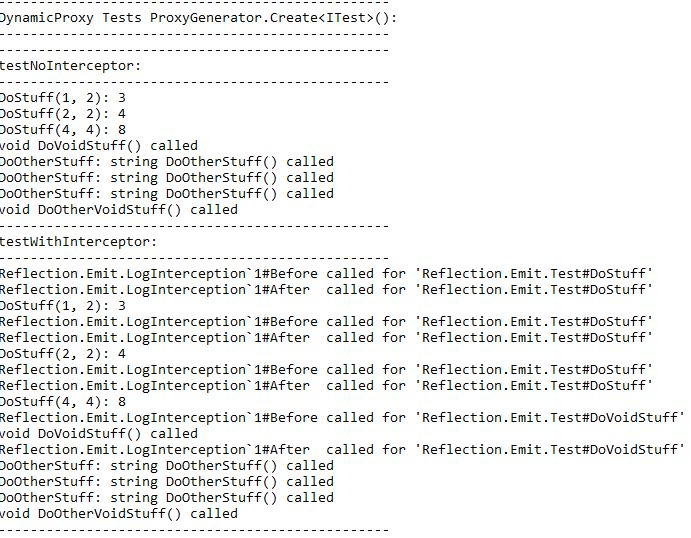
\includegraphics[scale=0.8]{\imageDir/test-proxy-generator_1.JPG}
	\caption{Test für \emph{Interception} von \emph{ITest}}
	\label{fig:image-proxy-generator}
\end{figure}
\ \newpage

\begin{figure}[h]
	\centering
	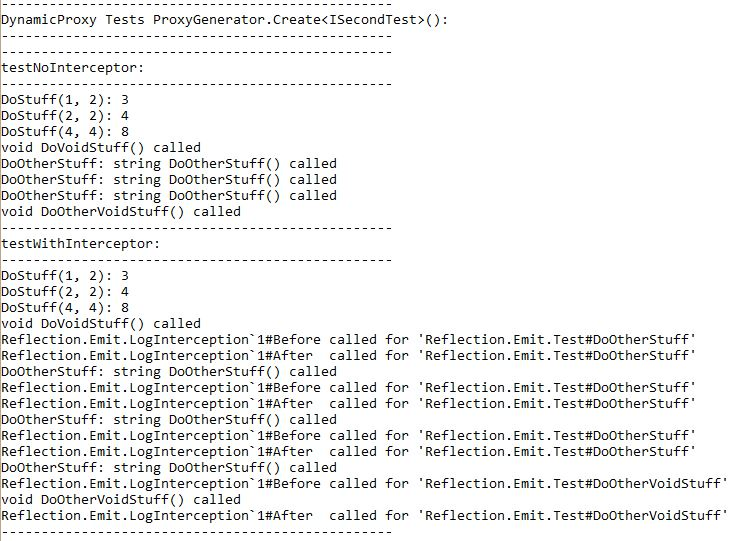
\includegraphics[scale=0.8]{\imageDir/test-proxy-generator_2.JPG}
	\caption{Test für \emph{Interception} von \emph{ISecondTest}}
	\label{fig:image-proxy-generator-2}
\end{figure}
\ \newpage

\begin{figure}[h]
	\centering
	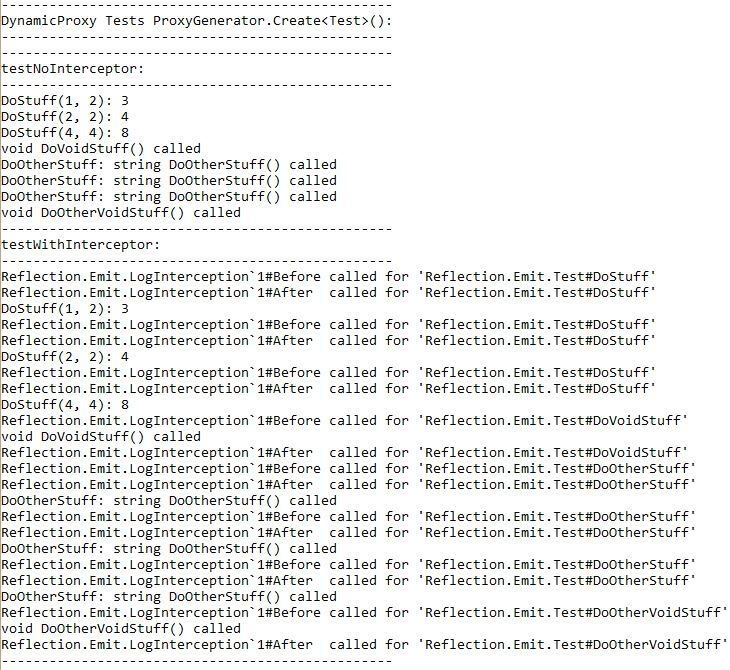
\includegraphics[scale=0.8]{\imageDir/test-proxy-generator_3.JPG}
	\caption{Test für \emph{Interception} von \emph{Test}}
	\label{fig:image-proxy-generator-2}
\end{figure}
\ \newpage

\section{Dynamic Generation of Functions}
Dieser Abschnitt behandelt die Aufgabenstellung \emph{Dynamic Generation of Functions}.

\subsection{Lösungsidee}
Ein Großteil der Implementierungen wurde bereits in der Übung implementiert, jedoch wurden die folgenden Veränderungen vorgenommen. 
\newline
\newline
Die Methode \emph{CompileTerminal} verlangt die Argumente in Form eines Strings Arrays und den Datentyp des Resultats der zu erzeugenden Methode, damit der Aufrufer nicht abhängig ist von statische Definitionen in der Implementierung dieser Methode.
\newline
\newline
Die Methode \emph{CompileFunction} verlangt das Argument in Form eines Strings und den Datentyp des Resultats der zu erzeugenden Methode, damit der Aufrufer nicht abhängig ist von statische Definitionen in der Implementierung dieser Methode.
\newline
\newline
Die \emph{delegate} Definitionen wurden in die Datei \emph{Node.cs} verschoben, da die \emph{delegates} die unterstützten Evaluierungsmethoden darstellen, die von den implementierten \emph{Nodes} unterstützt werden. Die Methoden \emph{CompileTerminal} und \emph{CompileFunctional} liefern ein Objekt des Datentyps \emph{T} und sind daher unabhängig von der konkreten Ausprägung der Terminal- und Funktionsmethode.  
\newline
\newline
Es wird die Schnittstelle \emph{INode} implementiert, die eine Node im Evaluierungsbaum darstellt. Es wird die abstrakte Klasse \emph{BaseNode} implementiert, die alle gemeinsamen \emph{Properties} kapselt. Es werden die Klassen \emph{FunctionalNode} und \emph{TerminalNode} implementiert, welche die Knoten der zwei Typen von Evaluierungsmethoden repräsentieren und die spezifischen Evaluierungen dieser Knotentypen implementieren. 

\subsection{Quelltexte}
Dieser Abschnitt beinhaltet die implementierten Quelltexte und das Testprogramm.
\begin{code}
	\caption{AssertDouble.cs}
	\cppSourceFile{\srcSymbolic/AssertDouble.cs}
	\label{src:class-assertdouble}
\end{code}

\begin{code}
	\caption{Node.cs}
	\cppSourceFile{\srcSymbolic/Node.cs}
	\label{src:class-inode-basenode-functional-node-terminal-node}
\end{code}

\begin{code}
	\caption{FunctionalBasis.cs}
	\cppSourceFile{\srcSymbolic/FunctionalBasis.cs}
	\label{src:class-functional-basis}
\end{code}

\begin{code}
	\caption{Program.cs}
	\cppSourceFile{\srcSymbolic/Program.cs}
	\label{src:class-symbolic-program}
\end{code}
\ \newpage

\subsection{Tests}
Dieser Abschnitt beinhaltet die implementierten Quelltexte und das Testprogramm.
\begin{figure}[h]
	\centering
	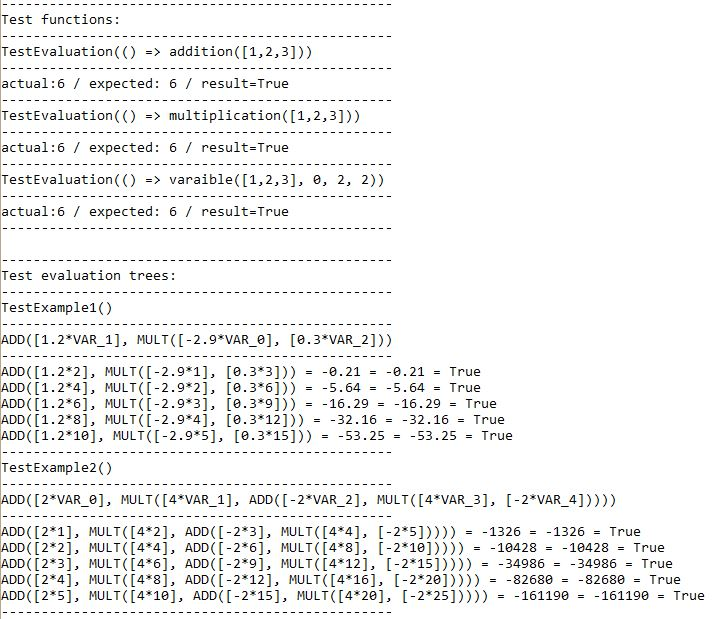
\includegraphics[scale=0.8]{\imageDir/test-symbolic-compuation.JPG}
	\caption{Ausgabe des Testprogramms}
	\label{fig:test-symbolic-compuation}
\end{figure}

\end{document}